%\documentclass{ExcelAtFIT}
%\documentclass[czech]{ExcelAtFIT} % when writing in CZECH
\documentclass[slovak]{ExcelAtFIT} % when writing in SLOVAK


%--------------------------------------------------------
%--------------------------------------------------------
%	REVIEW vs. FINAL VERSION
%--------------------------------------------------------

%   LEAVE this line commented out for the REVIEW VERSIONS
%   UNCOMMENT this line to get the FINAL VERSION
\ExcelFinalCopy


%--------------------------------------------------------
%--------------------------------------------------------
%	PDF CUSTOMIZATION
%--------------------------------------------------------

\hypersetup{
	pdftitle={Paper Title},
	pdfauthor={Author},
	pdfkeywords={Keyword1, Keyword2, Keyword3}
}

\lstset{
	backgroundcolor=\color{white},   % choose the background color; you must add \usepackage{color} or \usepackage{xcolor}; should come as last argument
	basicstyle=\footnotesize\tt,        % the size of the fonts that are used for the code
}

%--------------------------------------------------------
%--------------------------------------------------------
%	ARTICLE INFORMATION
%--------------------------------------------------------

\ExcelYear{2022}

\PaperTitle{Odhad pravdepodobnosti výskytu osôb v oblasti}

\Authors{Peter Koprda*}
\affiliation{*%
  \href{mailto:xkoprd00@stud.fit.vutbr.cz}{xkoprd00@stud.fit.vutbr.cz},
  \textit{Fakulta informačních technológií, Vysoké učení technické v Brně}}

\Keywords{Heat mapa --- Pravdepodobnosť výskytu osôb --- OpenStreetMap}

\Supplementary{N/A}


%--------------------------------------------------------
%--------------------------------------------------------
%	ABSTRACT and TEASER
%--------------------------------------------------------

\Abstract{
Cieľom práce je vytvoriť aplikáciu, ktorá na základe získaných mapových dát vytvorí odhady pravdepodobnosti výskytu osôb v určitej oblasti.
Odhad pravdepodobnosti výskytu osôb je zobrazený pomocou tzv. heat mapy. Heat mapa sa vytvára pomocou definovaných značiek (rôzne typy, napr.~poľná cesta, detské ihrisko), ktoré určujú, aký počet ľudí sa v danej oblasti nachádza. Každý typ značky má priradenú určitú pravdepodobnosť a podľa hodnôt pravdepodobností z~viacerých značiek je možné vytvoriť heat mapu. Výsledná heat mapa zobrazuje odhad pravdepodobnosti výskytu osôb v danej oblasti, ktorá nie vždy odráža realitu, pretože v niektorých menej významnejších oblastiach ani nedochádza k výskytu osôb z~dôvodu nízkej populácie.
Výsledkom práce je systém, ktorý môže slúžiť ako nástroj pri výstavbe elektroenergetických zariadení a elektrického vedenia u~ktorých môže dochádzať k ohrozeniu života, ak sa v~ich blízkosti nachádza osoba alebo osoby.
}

\Teaser{
    \TeaserImage{openstreetmap-logo.pdf}
    \TeaserImage{arrow.pdf}
    \TeaserImage{nahlad.png}
}



%--------------------------------------------------------
%--------------------------------------------------------
%--------------------------------------------------------
%--------------------------------------------------------
\begin{document}

\startdocument


%--------------------------------------------------------
%--------------------------------------------------------
%	ARTICLE CONTENTS
%--------------------------------------------------------

%--------------------------------------------------------
%--------------------------------------------------------
%--------------------------------------------------------
%--------------------------------------------------------
\section{Úvod}
Poruchy na \textit{elektroenergetických zariadeniach} - zariadenia, ktoré slúžia na výrobu, pripojenie, prenos, distribúciu alebo dodávku elektriny - nie sú ani v~dnešnej dobe nijako nezvyčajné. V~momente, keď sa stane porucha a v~blízkosti takéhoto zariadenia sa nachádza osoba, môže dôjsť k ohrozeniu života danej osoby. Pri poruche môže dôjsť ku zvýšeniu elektrického potenciálu na neživých častiach elektrického zariadenia a teda telom človeka začne prechádzať elektrický prúd~\cite{Vycital-Zemnisoustavy}. Aby sa predišlo zbytočným ohrozeniam života, je potrebné pomocou tzv. \emph{značiek} vytvoriť \emph{heat mapu}, ktorá sa používa na získanie hustoty domov, trestných činov apod.\cite{DeBoer-Heatmap}. Táto mapa by mala najvhodnejšie využitie mimo zastavaného územia, pretože v takomto území sa stavajú elektrické stožiare, ktoré majú najväčšiu pravdepodobnosť ohrozenia ľudského života. Na druhú stranu treba zohľadniť pri výstavbe elektroenergetických zariadení aj územné plány obcí, pretože iba pomocou mapových dát nie je možné zistiť, či z danej oblasti nebude v budúcnosti zastavaná plocha.

V dnešnej dobe zatiaľ neexistuje riešenie, ktoré by sa zaoberalo iba touto problematikou. Na získanie geografických dát je možné použiť otvorený projekt \emph{OpenStreetMap}~\cite{Openstreet}, z ktorých sa dá získať polohu elektroenergetických zariadení, ale neumožňuje pridávanie mapovej vrstvy s heat mapou. Kataster nehnuteľností, definovaný ako súbor údajov o nehnuteľnostiach, ktorý nám iba pomáha odhadnúť, na ktorých miestach sa nachádza väčší počet ľudí a~na ktorých menší počet ľudí. Z~územných plánov je možné získať informácie, kde sa nachádzajú resp.~kde sa budú nachádzať zastavané územia (ako je možné vidieť na obrázku \ref{fig:moravany}), avšak z~tohto územného plánu nie je možné získať informácie o~typoch ciest mimo zastavaného územia.

\begin{figure}[ht]
    \centering
    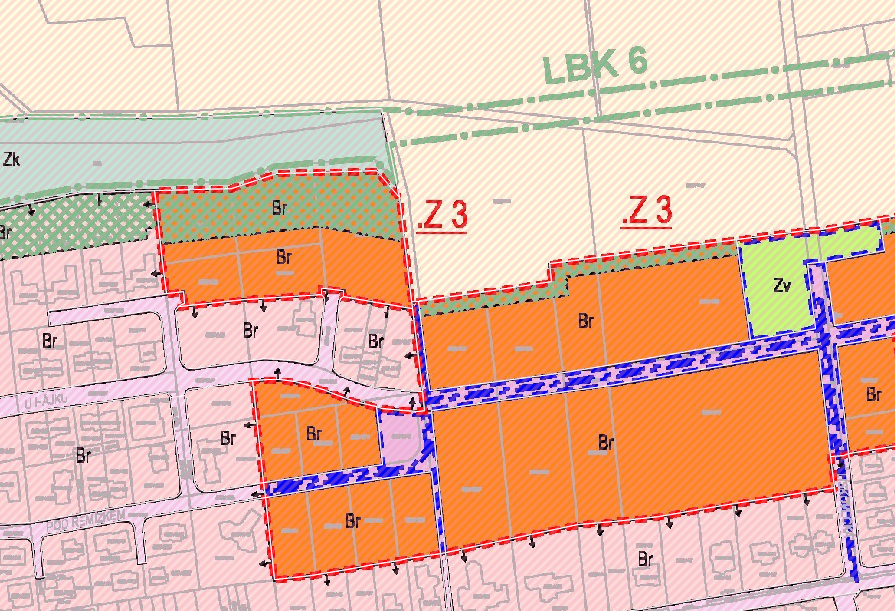
\includegraphics[width=0.9\linewidth]{images/jmk-uzemny-plan.png}
    \caption{Časť územného plánu obce Moravany. V~hornej časti obrázka sa nachádza poľnohospodárska plocha a v~dolnej časti obrázka sa nachádzajú plochy bývania. Zdroj:~\cite{Mapy-jmk}}
    \label{fig:moravany}
\end{figure}

Okrem OpenStreetMap a územných plánov obcí existujú GIS (Geografický Informačný Systém), ktoré sú schopné vytvárať heat mapy. Na druhú stranu je problém v tom, že tieto systémy sú často drahé a takisto je u nich problém vytvárať automaticky heat mapy zo získaných dát.

Riešením problému je vytvorenie heat mapy, ktorá zobrazuje pravdepodobnosť výskytu osôb v~určitej oblasti. Zdrojom pre vytvorenie heat mapy sú značky na mape, ktoré značia, aký objekt na mape sa nachádza: poľná cesta, detské ihrisko, autobusová stanica apod. Každá značka je zobrazovaná bodom resp. bodmi, ak značka predstavuje určitú cestu. Každý bod má svoj rádius, pričom v najbližšej vzdialenosti od daného bodu je pravdepodobnosť danej značky najvyššia a~so zvyšujúcou sa vzdialenosťou od daného bodu sa pravdepodobnosť lineárne zmenšuje. Druhým zdrojom pre riešenie tejto práce je použitie dát z územných plánov obcí.

Táto práca môže slúžiť pri výstavbe stožiarov na elektrické vedenie, ale aj na zhodnotenie rizík pri už postavených stožiaroch. Takisto predstavuje niektoré nové zdroje informácií, ktoré sa dajú získať pomocou mapových dát. V neposlednom rade môže táto práca slúžiť ako zdroj inšpirácie pre ostatných vývojárov a~to nielen z~OpenStreetMap komunity.


%--------------------------------------------------------
%--------------------------------------------------------
%--------------------------------------------------------
%--------------------------------------------------------
\section{Získavanie mapových dát}
\label{sec:ZiskavanieMapData}
Na získavanie mapových dát je možné použiť projekt OpenStreetMap~\cite{Openstreet}, čo je medzinárodný projekt vytvárajúci voľnú digitálnu mapu sveta. Tento projekt umožňuje pridávanie rôznych mapových vrstiev (napr. cyklomapa, dopravná mapa, humanitárna mapa), ale neumožňuje pridávanie vrstvy s heat mapou. Na to je vhodné použiť nástroje, ktoré takéto pridávanie vrstvy s heat mapou podporujú. Na získavanie mapových dát je možné použiť balíček nástrojov \texttt{OSMnx}\footnote{\url{https://osmnx.readthedocs.io}} z~jazyka Python, ktorý umožňuje sťahovanie geografických dát z~OpenStreetMap. Získané dáta sú vo formáte objektu typu \emph{GeoDataFrame}~\cite{Geopandas} \--- dvoj-dimenzionálna dátová štruktúra, podobná tabuľke s~riadkami a~stĺpcami. Táto dátová štruktúra je podtrieda \emph{pandas.DataFrame}\footnote{\url{https://pandas.pydata.org/docs/reference/api/pandas.DataFrame.html}} s~pridaným stĺpcom \texttt{geometry}. Najdôležitejšou vlastnosťou tejto dátovej štruktúry je to, že vždy má jeden \emph{GeoSeries} stĺpec, nazývaný ako \texttt{geometry} stĺpec. Tento stĺpec obsahuje geometrické objekty, pričom \emph{geopandas} má tri základné triedy geometrických objektov:
\begin{enumerate}
    \item Points / Multi-Points
    \item Lines / Multi-Lines
    \item Polygons / Multi-Polygons
\end{enumerate}

\begin{figure}[ht]
	\centering
	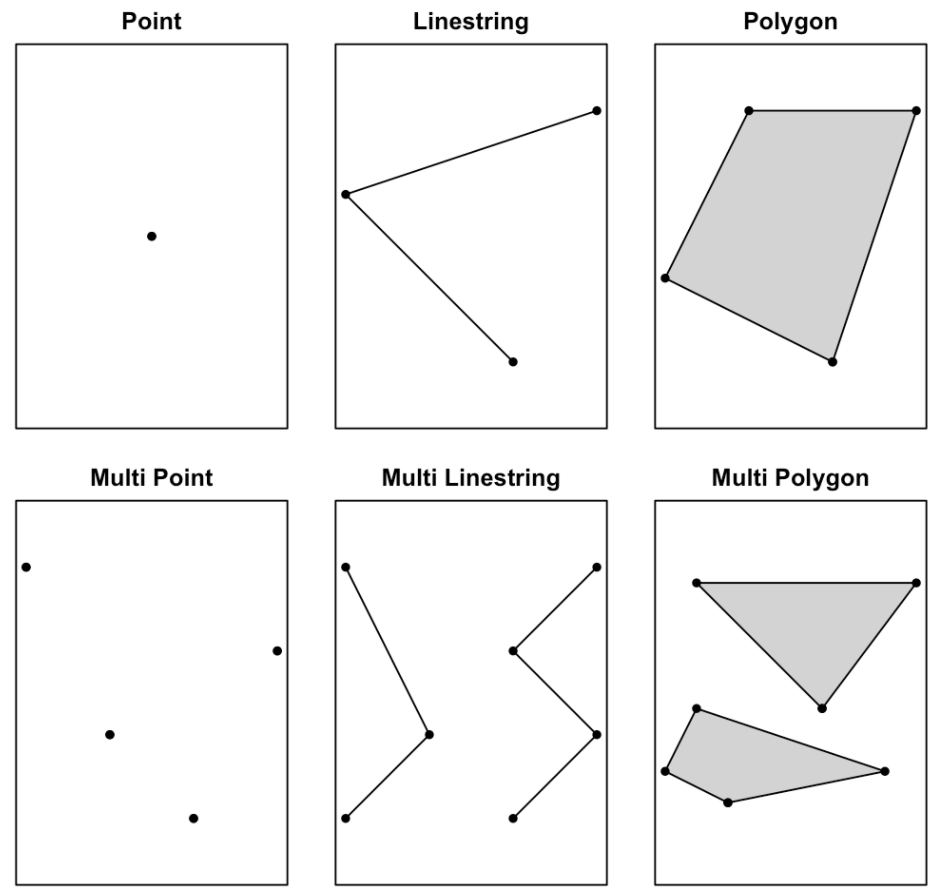
\includegraphics[width=0.9\linewidth]{images/geometric-types.png}
	\caption{Základné triedy geometrických objektov}
	\label{fig:GeometricTypes}
\end{figure}


%--------------------------------------------------------
%--------------------------------------------------------
%--------------------------------------------------------
%--------------------------------------------------------
\section{Vykresľovanie heat mapy}
\label{sec:VykreslovanieHeatmapy}
Heat mapa zobrazuje hustotu bodov v oblasti ako raster. Hustota bodových objektov je vypočítaná okolo každej výstupnej bunky rastru. Hodnota povrchu predstavuje pravdepodobnosť výskytu osoby pri danom bode. Pravdepodobnosť je najvyššia v mieste daného bodu a zmenšuje sa zväčšujúcou sa vzdialenosťou od~tohto miesta až k nulovej hodnote, ktorá je stanovená veľkosťou zvoleného polomeru. Pri prieniku viacerých bodov dochádza ku zvýšeniu hodnoty pravdepodobnosti v danom prieniku bodov, ako je možné vidieť na~obrázku~\ref{fig:HeatMapPoints}.

\begin{figure}[ht]
	\centering
	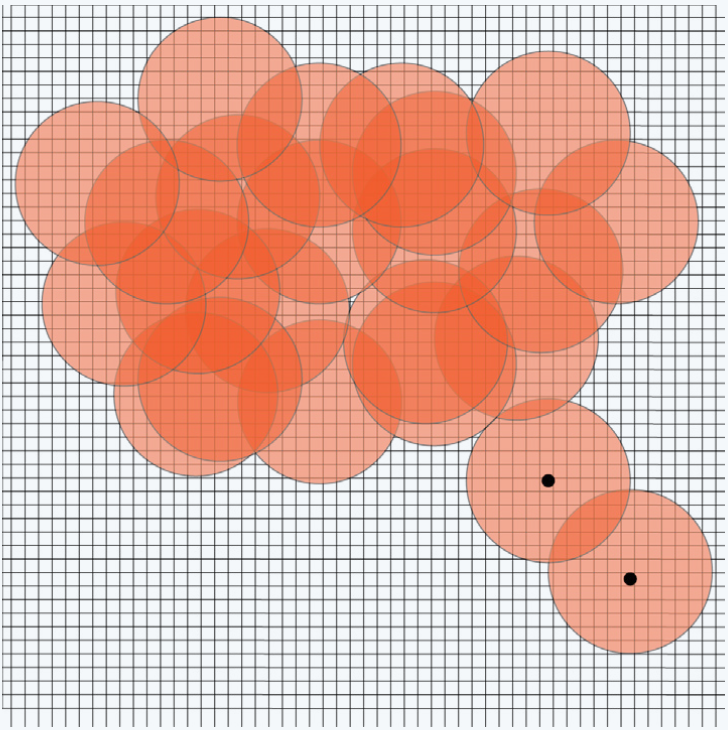
\includegraphics[width=0.9\linewidth]{images/heatmap-points.png}
	\caption{Prekrývajúce sa kružnice pri tvorbe heat mapy}
	\label{fig:HeatMapPoints}
\end{figure}

 Na to, aby bolo možné body na mapu vykresliť, je potrebné, aby každý bod mal definovanú svoju \emph{zemepisnú dĺžku} a~\emph{zemepisnú šírku} a aby mal definovaný polomer. Preto je potrebné, aby z geometrických objektov typu \emph{Line} a~\emph{Polygon} boli vytvorené geometrické objekty typu \emph{Point}, pretože tieto geometrické objekty majú definované iba hraničné body. 
 
 Cesta (typ Line), ktorá nemá zákruty, by sa bez úpravy vykreslil bod jedného konca cesty a bod druhého konca cesty. Takéto riešenie by nebolo vhodné, preto je potrebné použiť interpoláciu úsečky. Na interpoláciu úsečky je použitá rovnica \ref{eq:interpolate} odvodená z obrázka \ref{fig:Interpolation}:
\begin{linenomath}
    \begin{equation}
        y = y_1 + \frac{(x - x_1)(y_2 − y_1)}{x_2 − x_1},
        \label{eq:interpolate}
    \end{equation}
\end{linenomath}
kde $x_1$ a $y_1$ sú prvé súradnice, $x_2$ a $y_2$ sú druhé súradnice, $x$ je stredná hodnota hodnôt $x_1$ a $x_2$, a $y$ je hľadaná interpolovaná hodnota. Úsečku interpolujeme až dovtedy, dokým vzdialenosť medzi dvoma bodmi je väčšia ako zvolená hodnota $d$. Bez takejto interpolácie úsečiek by cesty nemali súvislú vrstvu heat mapy, t.j. iba časť cesty by bola pokrytá vrstvou heat mapy.
\begin{figure}[ht]
	\centering
	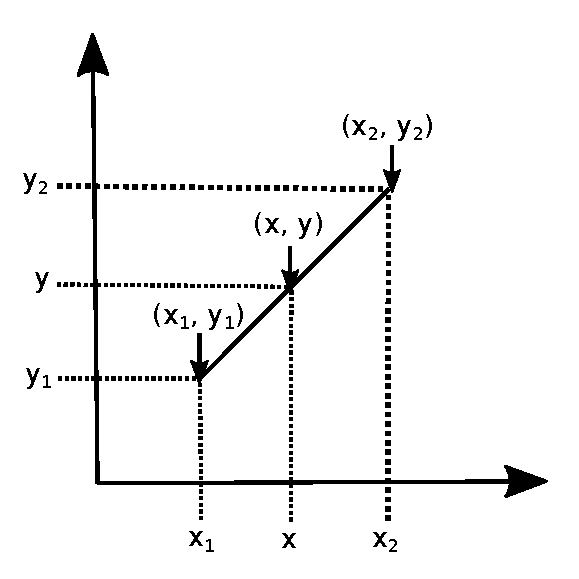
\includegraphics[width=0.75\linewidth]{images/linear-interpolation.pdf}
	\caption{Interpolácia úsečky}
	\label{fig:Interpolation}
\end{figure}

Budovy (typ Polygon) majú vyznačené iba okrajové body, vnútro tohto geometrického objektu je bez pomocných bodov. Na úpravu takýchto geometrických útvarov je potrebné použiť inú metódu ako sa použila u~ciest. Najlepším možným spôsobom by bolo získanie bodu, ktorý by bol priemerom všetkých bodov, ktoré tento geometrický objekt obsahuje. Na obrázku \ref{fig:Polygon} je možné vidieť, ako taký výpočet stredového bodu pre jednoduchý polygón \--- obdĺžnik \--- môže vyzerať. Je na ňom aj zobrazená pravdepodobnosť, vo vnútri celého polygónu je hodnota pravdepodobnosti rovnaká, ale mimo polygónu sa táto pravdepodobnosť lineárne zmenšuje až v určitom momente dosiahne hodnotu 0. Samozrejme, budovy majú rôzne tvary a u~niektorých je potrebné použiť zložitejšie úpravy.

\begin{figure}[ht]
	\centering
	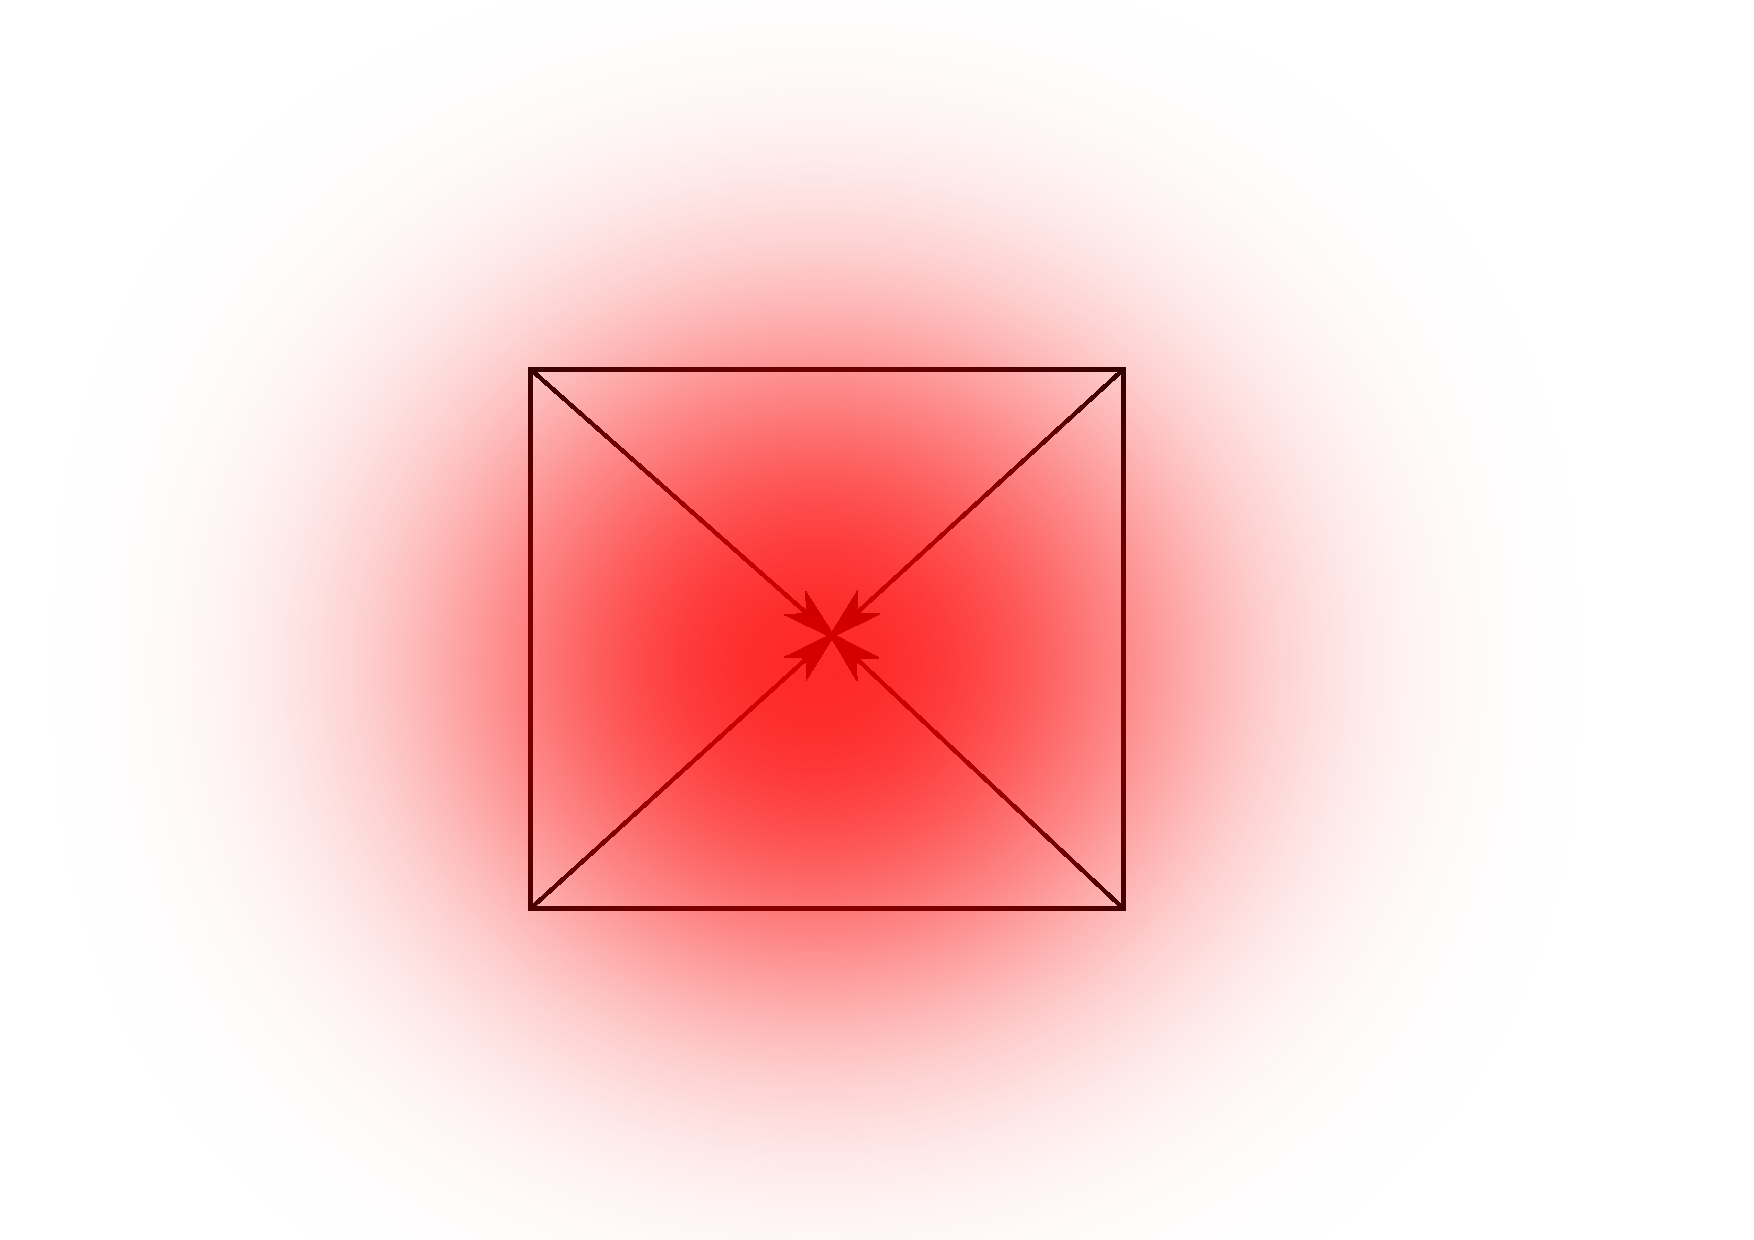
\includegraphics[width=0.8\linewidth]{images/heatmap-polygon.pdf}
	\caption{Zistenie stredového bodu}
	\label{fig:Polygon}
\end{figure}

Na vykresľovanie heat mapy je použitá knižnica \texttt{folium}, ktorá používa na pozadí knižnicu \texttt{Leaflet}\footnote{\url{https://leafletjs.com/}} z~jazyka JavaScript. Táto knižnica obsahuje triedu \texttt{HeatMap}, ktorá umožňuje vytvárať heat map vrstvu pre zadané vstupné parametre. Vstupnými parametrami by mal byť zoznam dvojíc \--- zemepisná dĺžka a zemepisná šírka alebo zoznam trojíc \--- zemepisná dĺžka, zemepisná šírka a váha. Váhe je priradená hodnota pravdepodobnosti, ktorú má daná značka. Okrem vstupných parametrov je možné pre tieto parametre zadefinovať vlastné argumenty, ktoré môžu byť:
\begin{itemize}
    \item \emph{min\_opacity} \--- minimálna nepriehľadnosť
    \item \emph{max\_zoom} \--- úroveň priblíženia, kedy body dosiahnu maximálnu intenzitu
    \item \emph{radius} \--- polomer každého bodu z heat mapy
    \item \emph{blur} \--- určuje, ako veľmi bod stráca farbu z teplej do studenej
    \item \emph{gradient} \---umožňuje vybrať farebnú schému
\end{itemize}


%--------------------------------------------------------
%--------------------------------------------------------
%--------------------------------------------------------
%--------------------------------------------------------
\section{Škála pre heat mapu}
\label{sec:Scale}
Každý objekt na mape môže mať rôznu pravdepodobnosť výskytu osôb. Preto bolo potrebné vytvoriť tabuľku, v ktorej sa nachádzajú všetky značky (resp. kľúče) na~označenie objektov na mape. Každý kľúč na mape môže nadobúdať rôzne hodnoty. Tieto hodnoty majú priradenú hodnotu pravdepodobnosti výskytu osôb. V~tabuľke~\ref{tab:Kluce} je možné vidieť niektoré kľúče s~hodnotami a~priradenými pravdepodobnosťami.

\begin{table}[h]
    \vskip6pt
    \caption{Tabuľka zoradená podľa hodnôt pravdepodobností}
    \centering
    \begin{tabular}{|c|c|c|c|}
        \hline
        \textbf{Kľúč} & \textbf{Hodnota} & \textbf{Popis} & {\textbf{P}} \\ \hline
        natural & volcano & Sopka & 0.1 \\ \hline
        highway & track & Lesná alebo poľná cesta & 0.3 \\ \hline
        building & tree\_house & Dom na strome & 0.6 \\ \hline
        amenity & bench & Lavička & 0.9 \\ \hline
        leisure & playground & Detské ihrisko & 1.0 \\ \hline
    \end{tabular}
    \label{tab:Kluce}
\end{table}

Táto tabuľka slúži ako podklad pre vytvorenie škály pre heat mapu ako aj podklad pre vytvorenie samotnej heat mapy. Kľúče s hodnotami s~najväčšou pravdepodobnosťou používajú teplé farby a~na~druhú stranu kľúče s~hodnotami s~najmenšou pravdepodobnosťou používajú studené farby. Hodnoty pravdepodobností neboli prevzaté a ani neboli získané experimentálne, pretože pri väčšom počte rôznorodých hodnôt pravdepodobností by to viedlo k tomu, že by sa musela s každou hodnotou pridať nová vrstva heat mapy. Keďže vrstvy danej mapy sa ukladajú na klientskej strane aplikácie, vytvorenie vrstiev heat mapy pri väčšom počte hodnôt pravdepodobností by viedlo zníženiu výkonu danej aplikácie.

\section{Experimenty}
\label{sec:Experimenty}
Experimenty sú vykonávané na rôznych častiach mapy, najčastejšie však na území Českej republiky. Aplikácia umožňuje vytvoriť mapu z plochy, ktoré je dané dvomi súradnicami zemepisnej dĺžky, severná a~južná, a~dvomi súradnicami zemepisnej dĺžky \--- východná a~západná.

Na obrázku~\ref{fig:Medlanky} je možné vidieť ako vyzerá heat mapa pre oblasť, v ktorej sa nachádzajú iba chaty (klúč: \texttt{building}, hodnota: \texttt{cabin}).

\begin{figure}[h]
    \centering
    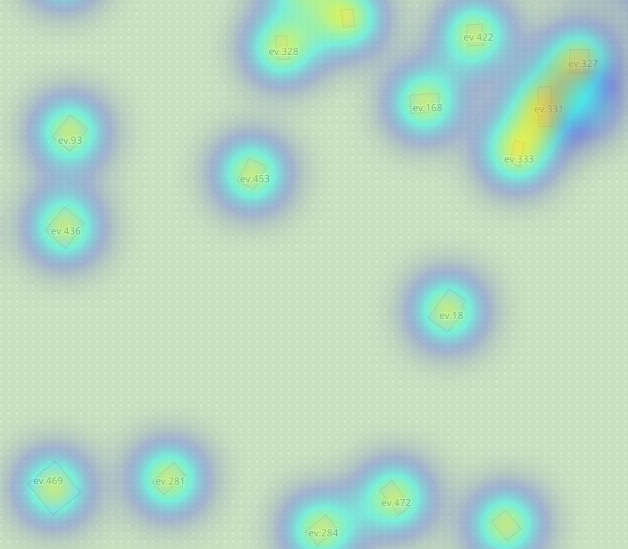
\includegraphics[width=0.8\linewidth]{images/brno-medlanky-heatmap.png}
    \caption{Heat mapa časti Brno-Medlánky.}
    \label{fig:Medlanky}
\end{figure}

Na obrázku~\ref{fig:Zabovresky} je možné vidieť, že dolná časť mapy obsahuje svetlejšie farby, pretože sa tam nachádzajú obytné domy. V strednej časti obrázka sa nachádzajú dve chatky, preto sú tam dva body v studenejšej farbe. V okolí týchto chatiek je pravdepodobnosť 0, preto okolie týchto chatiek je bezfarebné.

\begin{figure}[h]
	\centering
	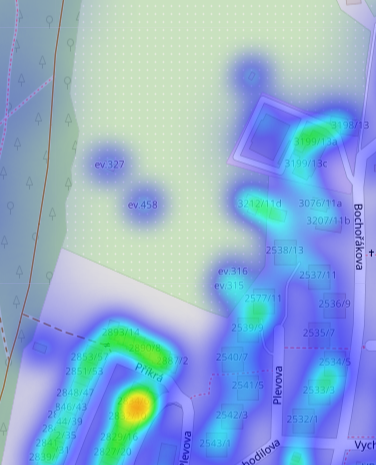
\includegraphics[width=0.8\linewidth]{images/brno-zabovresky-heatmap.png}
	\caption{Heat mapa časti Brno-Žabovřesky.}
	\label{fig:Zabovresky}
\end{figure}


Obrázok~\ref{fig:Medlanky} a obrázok~\ref{fig:Zabovresky} zobrazujú heat mapu, kde majú značky rovnakú pravdepodobnosť. Preto na lepšie zobrazenie výsledkov je vhodné použiť váhy \--- pravdepodobnosti. Heat mapa s~váhami pre dané značky je zobrazená na obrázku~\ref{fig:Rebesovice}, kde je možné vidieť, že na~rozdiel od ciest, ktoré majú vrstvu so studenejšími farbami, budovy v danej obci majú vrstvu s teplejšími farbami.

\begin{figure}[h]
    \centering
    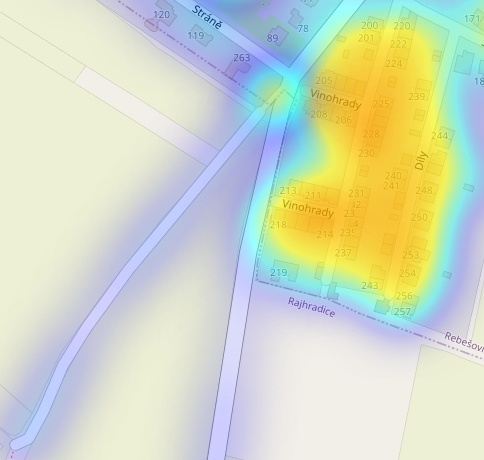
\includegraphics[width=1.0\linewidth]{images/rebesovice-heatmap.png}
    \caption{Heat mapa časti obce Rebešovice.}
    \label{fig:Rebesovice}
\end{figure}

%--------------------------------------------------------
%--------------------------------------------------------
%--------------------------------------------------------
%--------------------------------------------------------
\section{Záver}
\label{sec:Zaver}
Cieľom tejto práce bolo vytvoriť systém, ktorý by vedel odhadnúť pravdepodobnosť výskytu osôb v oblasti, ktorú zobrazuje pomocou heat mapy. Myslím, že práca účel splňuje, užívateľ je schopný získať heat mapu pre určitú oblasť. Závisí už len na dátach, či je vykreslená heat mapa relevantná. Mapové dáta sa veľmi líšia, v~celej krajine sa nachádzajú podobné budovy a~cesty, ale realita môže byť niekedy iná.

Získaná heat mapa môže slúžiť pri navrhovaní umiestnenia elektroenergetických zariadení, ktoré by mohli spôsobovať ujmu na zdraví, ak dôjde na takýchto zariadeniach k~poruche. V spolupráci s FEKT VUT bude možné tento systém použiť na zefektívnenie uzemnenia rozvodnej siete v Českej republike. Do budúcnosti by som chcel zauvažovať, ako by sa dali využiť dáta z územným plánov obcí. Takisto možným vhodným budúcim pridaním funkcionality by bolo užívateľské upravovanie heat mapy, ktoré by zlepšilo zobrazenú heat mapu.

\section*{Poďakovanie}
Chcel by som sa poďakovať predovšetkým pánovi Ing. Vojtěchovi Mrázekovi Ph.D. za jeho čas a cenné rady pri vedení tejto práce. Takisto by som sa chcel poďakovať pánovi doc. Ing. Davidovi Topolankovi, Ph.D. a pánovi  Ing. Václavovi Vyčítalovi Ph.D. za poskytnutie cenných informácií.

%--------------------------------------------------------
%--------------------------------------------------------
%--------------------------------------------------------
%	REFERENCE LIST
%--------------------------------------------------------
%--------------------------------------------------------
\phantomsection
\bibliographystyle{bib-styles/skplain.bst}
\bibliography{bibliography}

%--------------------------------------------------------
%--------------------------------------------------------
%--------------------------------------------------------
\end{document}